\documentclass{oblivoir}
    \usepackage{ikps}
    \usepackage{hyperref}
    \usepackage{graphicx}
\begin{document}

\title{\protect\sout{simple report} Not simple report}
\author{이윤승 201712052}
\maketitle
\tableofcontents

\section{build 과정}
참고 : \url{https://gracefulprograming.tistory.com/16}

\textbf{간략}
\begin{enumerate}
    \item 전처리 : .i 생성
    \item 컴파일 : .s 생성  어셈블러코드
    \item 어셈블리 .o 생성  기계어
    \item 링킹 .out 생성  실행파일
\end{enumerate}

\textbf{상세}

\begin{enumerate}
    \item 전처리 : .i 생성
    
    주체: 전처리기
    \begin{itemize}
        \item  해더 파일 삽입
        \item 매크로 치환 ,적용
    \end{itemize}
    \textbf{\#define}부분은 심볼테이블
    \footnote{\href{https://en.wikipedia.org/wiki/Symbol_table}{심볼테이블 참조}}
    에 저장해서 치환을 한다.(실제 심볼테이블이 어떻게 구성되는지는 모름, 테이블의 구현방식을 아예 모름)
    
    \item 컴파일 : .s 생성 전처리된 파일을 어셈블러코드로 만든다. 
    놀랍게도 컴파일 과정안에서 또 나뉜다

    \textbf{상상도 못한 정체!}

    \begin{figure}[h!]
        \centering
        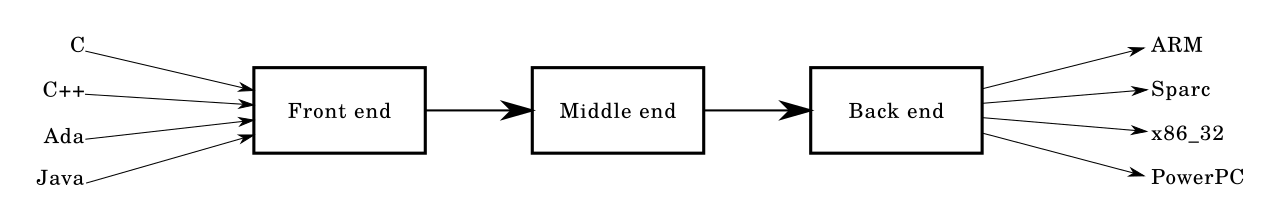
\includegraphics[scale = 0.3]{compiler.png}
    \end{figure}

    넘 복잡하고 어려워서 저도 잘 이해못함;;

    \begin{enumerate}
        \item 전단부(front-end) /*이 부분은 잘 이해못함 복붙 */ 
        
        \begin{figure}[h!]
            \centering
            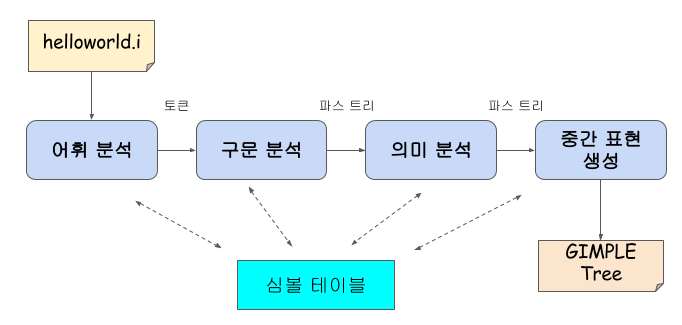
\includegraphics[scale = 0.5]{front.png}
        \end{figure}
        \begin{itemize}
            \item 어휘 분석: C 소스코드를 의미가 있는 최소단위(토큰 : Token)으로 나눕니다.
            \item 구문 분석: 토큰으로 파스 트리(Parse Tree)를 만들면서 문법적 오류를 검출합니다.
            \item 의미 분석: 파스 트리를 이용해 문법적 오류는 없지만 의미상 오류가 있는지 검사합니다. (함수의 매개변수를 잘못 사용했다거나 변수의 자료형(DataType)이 불일치 하는 것 등)
            \item 중간 표현 생성: 언어 독립적인 특성을 제공하기 위해 트리 형태의 중간표현(GIMPLE Tree)을 생성합니다.
        \end{itemize}
        \item 중단부(middle-end)

        \begin{figure}[h!]
            \centering
            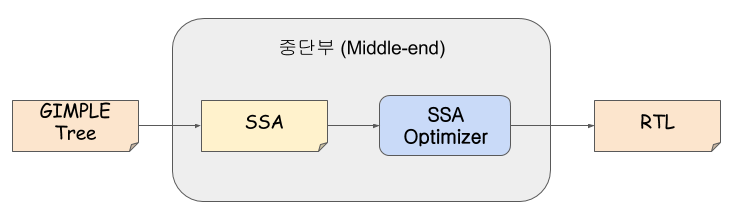
\includegraphics[scale = 0.5]{middle.png}
        \end{figure}

        SSA(Static Single Assignment)형태로 변환한 후에 아키텍쳐 비종속적인 최적화를 수행한 후 최종적으로 후단부에서 사용하는 RTL(Register Transfer Language: 고급 언어와 어셈블리 언어의 중간 형태

        \item 종단부(back-end)
        \begin{figure}[h!]
            \centering
            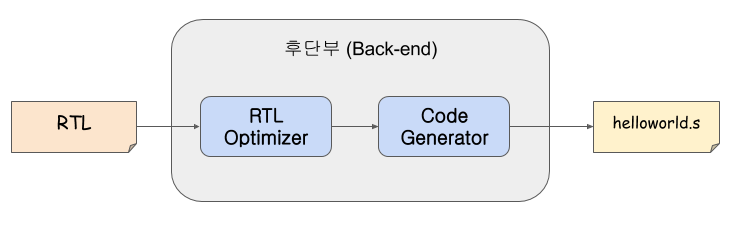
\includegraphics[scale = 0.5]{end.png}
        \end{figure}
        후단부에서는 RTL Optimizer에 의해 아키텍쳐 비종속적인 최적화와 함께 아키텍쳐 종속적인 최적화가 수행합니다. 

        아키텍쳐 종속적인 최적화는 각 프로그램 내의 명령어 중 아키텍처별로 좀 더 효율적인 명령어로 대체해 성능을 높이는 작업과 같이 아키텍쳐 특성에 따라 최적화를 수행하는 것을 말합니다.
        
        이렇게 최적화를 마치게 되면 Code Generator 어셈블리어로 구성된 .s 파일이 만들어지게 됩니다.
        
    \end{enumerate}

    \item 어셈블리 .o 생성
    주체: 어셈블러(assembler)
    컴파일, 어셈블리까지 하는 행위를 묶어서 컴파일 이러한 행위를 하는 주체를 compiler라고한다. 이 구간에서 나오는 아웃풋은 기계어로 나온다.

    여기까지해서 source code $\rightarrow$ object code 로 변환한다.
    \item 링킹 .out 생성 
    
    링킹을 해주는 주체를 링커라고하고 앞부분의 컴파일러와 링킹을 해주는 주체를 합쳐서 빌더라고 한다.
    간단하게 말하면 마지막으로 분할된 파일들을 모아 하나로 합쳐준다 그 파일들 중에서는 라이브러리, \href{https://en.wikipedia.org/wiki/Object_code}{obj}를 포함한다.
    1회차 수업 자료가 링킹에 대해 더 설명잘 되어있음
\end{enumerate}
%%%%%%%%%%%%%%%%%%%%%%%%%%%%%%%%%%%%%%%%%%%%%%%%%%%%%%%%%%%%%%

\section{linker와 headder file}

위의 빌드과정에서는 헤더 파일은 전혀 사용하지 않는다. 오직 소스파일 만을 사용하는데, 소스파일에서 인클루드 된 헤더파일은 단지 선언으로 이 클래스, 함수가 존재한다는것을 미리 알려줄 뿐, 전혀 해주는것이 없다. 하지만 컴파일러에게 있어서 현재 이 파일에는 정의가 되어있지 않지만 이 함수들이 다른 파일에 구현되어 있을 것이라는 것을 알려주고 일단 컴파일을 시킨뒤 링커를 통해서 적재적소에 붙여주는 일을 하게 해준다. 헤더파일(+ifndef로 주로 쓰는 대문자이름),구현 소스파일의 이름은 정말 자기마음대로 지어도 상관없다는 것을 알 수 있다. 프로젝트 안의 모든 파일들이 각각 알아서 컴파일되며 마지막 링커가 알아서 연결지어줄 뿐이다. \textbf{\#include}의 역할은 단순히 해당 코드를 그자리에 통째로 붙여주는 일밖에 하지않는다. 헤더파일의 역할을 다른 확장자명으로 해도 대신할수있지만\footnote{실제로 cpp로도 할수있음을 누군가의 과제로 보았을것이다.} 전통적으로 헤더파일로서 사용한다고 한다. 





\section{IDE()}
참고 : \url{http://www.qaupot.com/wordpress/?p=2048}







\section{ GCC compiler 사용}
참고 : \url{http://programmingskills.net/archives/278}






\section{template link error}
\subsection{why?}
왜 template을 쓰고 헤더 파일 분할을 하면 링크에러가 나는 걸까요?\\
필독 요망 : \url{https://www.tuwlab.com/ece/22227} \par

여기서 짚고 가야 할 중요한 사실이 하나 있는데, 바로 'Template Class는 Class가 아니다.' 라는 사실입니다. 이게 뭔소린가 하면, Template Class는 Class를 찍어내기 위한 '틀'일 뿐, Class 자체는 아니라는 것입니다.\par

컴파일러는 파일 단위로 컴파일을 진행하기 때문에 어떤 헤더파일이 어떤 소스파일과 짝인지 여부는 고려하지 않고 컴파일을 합니다. 그것도 헤더파일은 따로 컴파일하지 않으며, 컴파일 대상은 오직 소스파일들(*.c, *.cpp)뿐입니다.\par

소스파일에 헤더파일이 Include 되어 있다면, 헤더파일을 그대로 복붙하고 컴파일을 진행할 뿐입니다. 어떠한 소스파일에도 포함되지 않은 헤더파일이 존재한다면, 그 헤더파일은 컴파일되지 않습니다.(1주차 강의자료 참고)

\subsection{solution}
일단, \textbf{\#include}의 기본 작동 방식에 대해서 이해를 하고있어야 합니다. \\
참고: \url{http://www.sapphosound.com/archives/389}
\begin{enumerate}
    \item 기존에 .hpp에 쓰던 내용은 헤더파일 .h로 확장자명을 바꾼다.
    \item 기존에 .cpp에 쓰던 내용은 헤더파일 .hpp로 확장자명을 바꾼다 ( 헤더파일 폴더로 옮기는건 덤 )
    \item .h의 파일 마지막에 endif 직전에 \textbf{\#include "파일명.hpp"}를 붙인다
    \item  main 파일에는\textbf{\#include}" 파일명.h "를 한다.
    \item 짜잔!
\end{enumerate}
다른 방법으로는 기존에 똑같이 파일을 작성한후 ( hpp, cpp파일 두개로) \textbf{\#include}" 파일명.cpp "를 쓰면 됩니다.
물론 과제 3번에서 cpp 로 include 하면 뚝배기 깬다고 했으니 이렇게 안했습니다.


\url{http://programmingskills.net/archives/278}


\url{https://opentutorials.org/module/1594/9734}
\url{https://en.wikipedia.org/wiki/Compiler}
\end{document}
